\documentclass[a4paper,12pt,twoside]{memoir}

% Castellano
\usepackage[spanish,es-tabla]{babel}
\selectlanguage{spanish}
\usepackage[utf8]{inputenc}
\usepackage[T1]{fontenc}
\usepackage{lmodern} % Scalable font
\usepackage{microtype}
\usepackage{placeins}

\RequirePackage{booktabs}
\RequirePackage[table]{xcolor}
\RequirePackage{xtab}
\RequirePackage{multirow}


% Links
\PassOptionsToPackage{hyphens}{url}\usepackage[colorlinks]{hyperref}
\hypersetup{
	allcolors = {red}
}

% Ecuaciones
\usepackage{amsmath}

% Rutas de fichero / paquete
\newcommand{\ruta}[1]{{\sffamily #1}}

% Párrafos
\nonzeroparskip

% Huérfanas y viudas
\widowpenalty100000
\clubpenalty100000

% Imágenes

% Comando para insertar una imagen en un lugar concreto.
% Los parámetros son:
% 1 --> Ruta absoluta/relativa de la figura
% 2 --> Texto a pie de figura
% 3 --> Tamaño en tanto por uno relativo al ancho de página
\usepackage{graphicx}
\newcommand{\imagen}[3]{
	\begin{figure}[!h]
		\centering
		\includegraphics[width=#3\textwidth]{#1}
		\caption{#2}\label{fig:#1}
	\end{figure}
	\FloatBarrier
}

% Comando para insertar una imagen sin posición.
% Los parámetros son:
% 1 --> Ruta absoluta/relativa de la figura
% 2 --> Texto a pie de figura
% 3 --> Tamaño en tanto por uno relativo al ancho de página
\newcommand{\imagenflotante}[3]{
	\begin{figure}
		\centering
		\includegraphics[width=#3\textwidth]{#1}
		\caption{#2}\label{fig:#1}
	\end{figure}
}

% El comando \figura nos permite insertar figuras comodamente, y utilizando
% siempre el mismo formato. Los parametros son:
% 1 --> Porcentaje del ancho de página que ocupará la figura (de 0 a 1)
% 2 --> Fichero de la imagen
% 3 --> Texto a pie de imagen
% 4 --> Etiqueta (label) para referencias
% 5 --> Opciones que queramos pasarle al \includegraphics
% 6 --> Opciones de posicionamiento a pasarle a \begin{figure}
\newcommand{\figuraConPosicion}[6]{%
  \setlength{\anchoFloat}{#1\textwidth}%
  \addtolength{\anchoFloat}{-4\fboxsep}%
  \setlength{\anchoFigura}{\anchoFloat}%
  \begin{figure}[#6]
    \begin{center}%
      \Ovalbox{%
        \begin{minipage}{\anchoFloat}%
          \begin{center}%
            \includegraphics[width=\anchoFigura,#5]{#2}%
            \caption{#3}%
            \label{#4}%
          \end{center}%
        \end{minipage}
      }%
    \end{center}%
  \end{figure}%
}

%
% Comando para incluir imágenes en formato apaisado (sin marco).
\newcommand{\figuraApaisadaSinMarco}[5]{%
  \begin{figure}%
    \begin{center}%
    \includegraphics[angle=90,height=#1\textheight,#5]{#2}%
    \caption{#3}%
    \label{#4}%
    \end{center}%
  \end{figure}%
}
% Para las tablas
\newcommand{\otoprule}{\midrule [\heavyrulewidth]}
%
% Nuevo comando para tablas pequeñas (menos de una página).
\newcommand{\tablaSmall}[5]{%
 \begin{table}
  \begin{center}
   \rowcolors {2}{gray!35}{}
   \begin{tabular}{#2}
    \toprule
    #4
    \otoprule
    #5
    \bottomrule
   \end{tabular}
   \caption{#1}
   \label{tabla:#3}
  \end{center}
 \end{table}
}

%
% Nuevo comando para tablas pequeñas (menos de una página).
\newcommand{\tablaSmallSinColores}[5]{%
 \begin{table}[H]
  \begin{center}
   \begin{tabular}{#2}
    \toprule
    #4
    \otoprule
    #5
    \bottomrule
   \end{tabular}
   \caption{#1}
   \label{tabla:#3}
  \end{center}
 \end{table}
}

\newcommand{\tablaApaisadaSmall}[5]{%
\begin{landscape}
  \begin{table}
   \begin{center}
    \rowcolors {2}{gray!35}{}
    \begin{tabular}{#2}
     \toprule
     #4
     \otoprule
     #5
     \bottomrule
    \end{tabular}
    \caption{#1}
    \label{tabla:#3}
   \end{center}
  \end{table}
\end{landscape}
}

%
% Nuevo comando para tablas grandes con cabecera y filas alternas coloreadas en gris.
\newcommand{\tabla}[6]{%
  \begin{center}
    \tablefirsthead{
      \toprule
      #5
      \otoprule
    }
    \tablehead{
      \multicolumn{#3}{l}{\small\sl continúa desde la página anterior}\\
      \toprule
      #5
      \otoprule
    }
    \tabletail{
      \hline
      \multicolumn{#3}{r}{\small\sl continúa en la página siguiente}\\
    }
    \tablelasttail{
      \hline
    }
    \bottomcaption{#1}
    \rowcolors {2}{gray!35}{}
    \begin{xtabular}{#2}
      #6
      \bottomrule
    \end{xtabular}
    \label{tabla:#4}
  \end{center}
}

%
% Nuevo comando para tablas grandes con cabecera.
\newcommand{\tablaSinColores}[6]{%
  \begin{center}
    \tablefirsthead{
      \toprule
      #5
      \otoprule
    }
    \tablehead{
      \multicolumn{#3}{l}{\small\sl continúa desde la página anterior}\\
      \toprule
      #5
      \otoprule
    }
    \tabletail{
      \hline
      \multicolumn{#3}{r}{\small\sl continúa en la página siguiente}\\
    }
    \tablelasttail{
      \hline
    }
    \bottomcaption{#1}
    \begin{xtabular}{#2}
      #6
      \bottomrule
    \end{xtabular}
    \label{tabla:#4}
  \end{center}
}

%
% Nuevo comando para tablas grandes sin cabecera.
\newcommand{\tablaSinCabecera}[5]{%
  \begin{center}
    \tablefirsthead{
      \toprule
    }
    \tablehead{
      \multicolumn{#3}{l}{\small\sl continúa desde la página anterior}\\
      \hline
    }
    \tabletail{
      \hline
      \multicolumn{#3}{r}{\small\sl continúa en la página siguiente}\\
    }
    \tablelasttail{
      \hline
    }
    \bottomcaption{#1}
  \begin{xtabular}{#2}
    #5
   \bottomrule
  \end{xtabular}
  \label{tabla:#4}
  \end{center}
}



\definecolor{cgoLight}{HTML}{EEEEEE}
\definecolor{cgoExtralight}{HTML}{FFFFFF}

%
% Nuevo comando para tablas grandes sin cabecera.
\newcommand{\tablaSinCabeceraConBandas}[5]{%
  \begin{center}
    \tablefirsthead{
      \toprule
    }
    \tablehead{
      \multicolumn{#3}{l}{\small\sl continúa desde la página anterior}\\
      \hline
    }
    \tabletail{
      \hline
      \multicolumn{#3}{r}{\small\sl continúa en la página siguiente}\\
    }
    \tablelasttail{
      \hline
    }
    \bottomcaption{#1}
    \rowcolors[]{1}{cgoExtralight}{cgoLight}

  \begin{xtabular}{#2}
    #5
   \bottomrule
  \end{xtabular}
  \label{tabla:#4}
  \end{center}
}



\graphicspath{ {./img/} }

% Capítulos
\chapterstyle{bianchi}
\newcommand{\capitulo}[2]{
	\setcounter{chapter}{#1}
	\setcounter{section}{0}
	\setcounter{figure}{0}
	\setcounter{table}{0}
	\chapter*{\thechapter.\enskip #2}
	\addcontentsline{toc}{chapter}{\thechapter.\enskip #2}
	\markboth{#2}{#2}
}

% Apéndices
\renewcommand{\appendixname}{Apéndice}
\renewcommand*\cftappendixname{\appendixname}

\newcommand{\apendice}[1]{
	%\renewcommand{\thechapter}{A}
	\chapter{#1}
}

\renewcommand*\cftappendixname{\appendixname\ }

% Formato de portada
\makeatletter
\usepackage{xcolor}
\newcommand{\tutor}[1]{\def\@tutor{#1}}
\newcommand{\course}[1]{\def\@course{#1}}
\definecolor{cpardoBox}{HTML}{E6E6FF}
\def\maketitle{
  \null
  \thispagestyle{empty}
  % Cabecera ----------------
\noindent
\includegraphics[width=\textwidth]{cabecera}\vspace{1cm}%
  \vfill
  % Título proyecto y escudo informática ----------------
  \colorbox{cpardoBox}{%
    \begin{minipage}{.8\textwidth}
      \vspace{.5cm}\Large
      \begin{center}
      \textbf{TFG del Grado en Ingeniería Informática}\vspace{.6cm}\\
      \textbf{\LARGE\@title{}}
      \end{center}
      \vspace{.2cm}
    \end{minipage}

  }%
  \hfill\begin{minipage}{.20\textwidth}
    
\includegraphics[width=\textwidth]{escudoInfor}
  \end{minipage}
  \vfill
  % Datos de alumno, curso y tutores ------------------
  \begin{center}%
  {%
    \noindent\LARGE
    Presentado por \@author{}\\ 
    en Universidad de Burgos --- \@date{}\\
    Tutor: \@tutor{}\\
  }%
  \end{center}%
  \null
  \cleardoublepage
  }
\makeatother

\newcommand{\nombre}{David Martínez Bahillo} %%% cambio de comando

% Datos de portada
\title{ContractMe}
\author{\nombre}
\tutor{Sandra Rodriguez Arribas}
\date{\today}

\begin{document}

\maketitle


\newpage\null\thispagestyle{empty}\newpage


%%%%%%%%%%%%%%%%%%%%%%%%%%%%%%%%%%%%%%%%%%%%%%%%%%%%%%%%%%%%%%%%%%%%%%%%%%%%%%%%%%%%%%%%
\thispagestyle{empty}


\noindent
\includegraphics[width=\textwidth]{cabecera}\vspace{1cm}

\noindent Dña. Sandra Rodríguez Arribas , profesora del departamento de ingeniería informática, área de lenguajes y sistemas informáticos.

\noindent Expone:

\noindent Que el alumno D. \nombre, con DNI 71566321G, ha realizado el Trabajo final de Grado en Ingeniería Informática titulado <<ContractMe>>. 

\noindent Y que dicho trabajo ha sido realizado por el alumno bajo la dirección del que suscribe, en virtud de lo cual se autoriza su presentación y defensa.

\begin{center} %\large
En Burgos, {\large \today}
\end{center}

\vfill\vfill\vfill

% Author and supervisor
%\begin{minipage}{0.45\textwidth}
%\begin{flushleft} %\large
%Vº. Bº. del Tutor:\\[2cm]
%D. nombre tutor
%\end{flushleft}
%\end{minipage}
%\hfill
%\begin{minipage}{0.45\textwidth}
%\begin{flushleft} %\large
%Vº. Bº. del co-tutor:\\[2cm]
%D. nombre co-tutor
%\end{flushleft}
%\end{minipage}
%\hfill

%\vfill

% para casos con solo un tutor comentar lo anterior
% y descomentar lo siguiente
Vº. Bº. del Tutor:\\[2cm]
Sandra Rodríguez Arribas


\newpage\null\thispagestyle{empty}\newpage




\frontmatter

% Abstract en castellano
\renewcommand*\abstractname{Resumen}
\begin{abstract}

Este proyecto se enfoca en la creación de una solución innovadora para la contratación laboral, aprovechando la tecnología \textit{blockchain} y los contratos inteligentes. Se busca agilizar el proceso de contratación en sectores como la agricultura y servicios domésticos mediante la automatización de la gestión de contratos desde su inició hasta su final.
El proyecto incorpora métodos de autenticación biométrica y escaneo de códigos QR, apoyándose en soluciones de identidad descentralizadas para proteger la privacidad de los usuarios.

El objetivo final es proporcionar una herramienta que promueva prácticas de empleo transparentes y legales, optimizando los procesos de contratación y verificación para empleadores y trabajadores garantizando la seguridad de todos los trámites.

\end{abstract}

\renewcommand*\abstractname{Descriptores}
\begin{abstract}

\textit{Blockchain}, contratos inteligentes, autenticación biométrica, aplicación móvil, procesamiento pagos.

\end{abstract}

\clearpage

% Abstract en inglés
\renewcommand*\abstractname{Abstract}
\begin{abstract}
This project focuses on creating an innovative solution for labor recruitment, taking advantage of blockchain technology and smart contracts. The aim is to streamline the contracting process in sectors such as agriculture and domestic services by automating contract management from start to finish.
The project incorporates biometric authentication methods and QR code scanning, relying on decentralized identity solutions to protect user privacy.

The ultimate goal is to provide a tool that promotes transparent and legal employment practices, optimizing the hiring and verification processes for employers and workers, guaranteeing the security of all procedures.

\end{abstract}

\renewcommand*\abstractname{Keywords}
\begin{abstract}

Blockchain, smart contracts, biometric authentication, mobile app, payment processing.

\end{abstract}

\clearpage

% Indices
\tableofcontents

\clearpage

\listoffigures

\clearpage

\listoftables
\clearpage

\mainmatter
\capitulo{1}{Introducción}

La transformación digital se ha convertido en un pilar fundamental para el desarrollo y la eficiencia de diversos sectores económicos, entre ellos el mercado laboral. Sin embargo, a pesar de los avances tecnológicos, ciertos sectores como la agricultura, los servicios domésticos y el trabajo freelance enfrentan retos significativos en la gestión eficiente de contrataciones y la verificación de identidad y tiempo laboral.
Estos desafíos se ven agravados por la presencia de la economía sumergida, donde la falta de transparencia y la informalidad laboral no solo perjudican la economía global, sino que también vulneran los derechos de los trabajadores.
En este contexto, se pretende implementar una solución innovadora que permita superar las barreras existentes, haciendo frente a la economía sumergida mediante el empleo de tecnologías disruptivas como blockchain y contratos inteligentes. Esta iniciativa busca promover la formalización de empleos y asegurar prácticas laborales justas, abordando directamente los problemas de falta de transparencia y seguridad en los procesos contractuales. Se destacará el impacto social y económico de reducir la economía sumergida, apoyándose en datos que evidencian su magnitud y las implicaciones positivas de una mayor formalización laboral.

La adopción de contratos inteligentes en una red blockchain permite una gestión contractual transparente, segura y automática, asegurando que los términos acordados se cumplan eficazmente sin intervención manual.
Esta tecnología también proporciona un registro inmutable y verificable de las transacciones y acuerdos labores, combatiendo así prácticas ilegales y fomentando un entorno de trabajo más equitativo.

Este proyecto no solo aborda la necesidad de un sistema de contratación y verificación más eficiente y seguro sino que también se anticipa a las demandas de un mercado laboral en constante evolución, ofreciendo una herramienta adaptable y escalable. Con una interfaz de usuario diseñada para la simplicidad y la accesibilidad en dispositivos móviles, se busca fomentar prácticas de empleo legales y transparentes, contribuyendo a la creación de un entorno laboral más justo y seguro para todos.
La inclusión de tecnologías GPS y la autenticación biométrica refuerza este objetivo, permitiendo un seguimiento preciso de las horas de trabajo y asegurando la identidad de los trabajadores de manera segura y privada.

Por tanto este proyecto no solo propone una solución práctica que beneficia tanto a trabajadores como empleadores, sino que también tiene el potencial de impactar positivamente en la economía global. marcando un paso adelante hacia la erradicación de la economía sumergida y el establecimiento de prácticas laborales más justas y transparentes a nivel mundial.
\capitulo{2}{Objetivos del proyecto}

En esta sección se muestran las metas que se pretenden alcanzar con el desarrollo del proyecto.

\section*{Objetivos técnicos}

\begin{enumerate}

\item \textbf{Seguir estándares en el desarrollo de contratos inteligentes}: Alineándose con las mejores prácticas de la comunidad Ethereum y Solidity. 

\item \textbf{Adoptar metodologías ágiles}: Para favorecer un desarrollo iterativo y eficiente, facilitando la adaptación a cambios y mejora continua del proyecto.

\item \textbf{Documentar del proyecto}: Utilizando herramientas visuales para explicar la arquitectura. 

\item \textbf{Mantener un alto estándar de calidad en el código}: Empleando herramientas de revisión de código.


\item \textbf{Evaluar la calidad de la solución}: En términos de eficiencia.

\item \textbf{Planear un plan de implementeción y escalabilidad}

\end{enumerate}


%DEBERÍA METER ALGO SOBRE LA BASE DE DATOS??
\section*{Objetivos del Software}

\begin{enumerate}

\item \textbf{Integrar Ethereum en el proyecto}: Asegurando una implementación efectiva para el despliegue de contratos inteligentes

\item \textbf{Desarrollar contratos inteligentes con Solidity}: Asegurando un código eficiente y adaptado a las necesidades específicas de la contratación laboral. 

\item \textbf{Desplegar en una red Ethereum real}: Logrando una convivencia con el resto de contratos de la comunidad.

\item \textbf{Implementar tecnologías de autenticación biométrica}: Utilizando métodos como la huella dactilar o el reconocimiento facial para la identificación del usuario.

\item \textbf{Integrar tecnología GPS}: Verificando la presencia del trabajador en el lugar adecuado y el momento correcto.

\item \textbf{implementar códigos QR}: Agilizando los procesos administrativos y operativos además de aplicar una capa adicional de seguridad.

\item \textbf{Integrar servicios de inicio sesión}: Proporcionando a los usuarios opciones de inicio de sesión descentralizadas a través de MetaMask.

\item \textbf{Desarrollar una interfaz de usuario intuitiva y accesible}: Priorizando la simplicidad y la usabilidad para garantizar una plataforma fácil de utilizar para todos los usuarios.



\end{enumerate}
\capitulo{3}{Conceptos teóricos}

En esta sección se sintetizarán algunos conceptos teóricos relevantes para la correcta compresión del proyecto.

\section{Introducción a la \textit{blockchain}}

La \textit{blockchain} proporciona un registro inmutable y en tiempo real de transacciones, emergió como una solución al problema de doble gasto~\cite{dobleGasto} en transacciones digitales, un desafío que había eludido a los criptógrafos durante décadas, el cual consiste en la posibilidad de gastar una misma moneda digital más de una vez. Esto ocurre debido a la falsificación o duplicación de archivos digitales que representan la moneda.
En 2008 una persona o grupo anónimo, bajo el seudónimo de Satoshi Nakamoto, publicó un documento técnico para crear una moneda digital para contabilizar y transferir valor. Así nació una tecnología que se fundamenta en una base de datos descentralizada compuesta por bloques de información replicados y sincronizados en múltiples ordenadores.  
Esta premisa hizo que en enero de 2009 entrara en funcionamiento la primera red basada en el protocolo Bitcoin~\cite{introducciónBitcoin}.
La \textit{blockchain} demostró su capacidad para contabilizar y transferir valor de manera segura sin la necesidad de intermediarios, transformando el sector financiero y encontrando aplicaciones en una variedad de industrias.



\section{Tecnología subyacente}


\subsection{Nodo}

Los nodos en \textit{blockchain} son dispositivos, generalmente computadoras, que participan en una red \textit{blockchain}. Estos dispositivos ejecutan el software del protocolo \textit{blockchain}, lo que les permite ayudar a validar transacciones y mantener la seguridad de la red~\cite{IntroducciónNodo}.

Para lograr esto, los nodos se comunican entre sí por medio de protocolos \textit{peer-to-peer}(P2P). En un sistema P2P, cada nodo se conecta directamente a otros nodos sin necesidad de intermediarios. Cada nodo actúa tanto como cliente como servidor, compartiendo la carga de procesamiento de datos y la transmisión de información.
Esta arquitectura (ver imagen ~\ref{fig:BCdescentralizada}) permite desarrollar un red robusta y descentralizada donde cada nodo contribuye al mantenimiento y seguridad de la red. Siendo extremadamente difícil censurar o bloquear el acceso a la red, ya que no hay un punto central de control.

\begin{figure}[h]
	\centering
	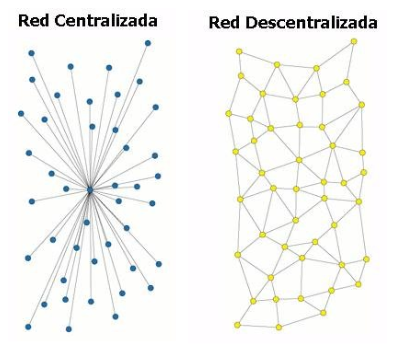
\includegraphics[width=0.75\textwidth]{BCdescentralizada}
	\caption[Tipos de redes]{Diferencias entre una red centralidad y descentralizada~\cite{tiposRedes}.}
	\label{fig:BCdescentralizada}
\end{figure}


Resulta fundamental comprender los distintos tipos de nodos que conviven en una red y el papel específico que cada uno desempeña. A continuación, se enumerarán los tipos de nodos, destacando sus características y funciones únicas~\cite{tiposNodos}.

\begin{itemize}
\item \textbf{Nodos completos:} Estos nodos albergan una copia completa del libro mayor de la \textit{blockchain}. Al contener el registro completo de todas las transacciones, los nodos pueden verificar de forma independiente cualquier transacción sin necesidad de recurrir a información externa.

\item \textbf{Nodos ligeros:} Han sido diseñados para dispositivos con recursos limitados, los nodos ligeros no almacenan el registro completo, sino que confían en los nodos completos para obtener dicha información.

\item \textbf{Nodos mineros:} Son utilizados en las redes que utilizan el algoritmo de consenso Proof of Work(PoW), los nodos mineros compiten para agregar nuevos bloques a la \textit{blockchain} para obtener una recompensa por ello.

\item \textbf{Nodos completos podados:} Estos nodos almacenan una versión recortada del registro, eliminando datos antiguos para ahorrar espacio, pero a diferencia de los nodos ligeros estos pueden seguir verificando de forma independiente cualquier transacción. 

\item \textbf{Nodos completos de archivo:} Almacenan todo el libro mayor del \textit{blockchain}, desde el principio de los tiempos. Los nodos completos de archivo son la única fuente valiosa y fiable para verificar los datos de transacciones anteriores en la historia de una \textit{blockchain}, ya que no están afectados por el límite de tiempo o almacenamiento.
A diferencia de los nodos completos, los nodos de archivo vas más allá al almacenar cada cambio de estado en la \textit{blockchain}.

\item \textbf{Nodos de autoridad:} Utilizados en \textit{blockchains} con mecanismos de consenso como Proof of Authority(PoA), estos nodos son operados por entidades verificadas y de confianza dentro de la red. A diferencia de PoW, tienen el poder de validar bloques sin necesidad de competir entre ellos.

\item \textbf{Nodos maestros:} Ofrecen funcionalidades adicionales como la ejecución de contratos inteligentes. Requieren de una garantía o \textit{stake} para operar y suelen recibir incentivos por ofrecer servicios especializados.

\item \textbf{Nodos de estaca:} Utilizados en \textit{blockchains} que funcionan con el algoritmo de consenso Proof of Stake(PoS) donde los nodos participan en la validación de bloques apostando una cierta cantidad de criptomonedas como garantía para operar.

\item \textbf{Nodos \textit{Lightning}:} Específicos de las soluciones de segunda capa como \textit{Lightning Network}, estos nodos facilitan transacciones rápidas y de bajo costo fuera de la cadena principal, ayudando a reducir la congestión.

\item \textbf{Supernodos:} Son nodos con capacidades y responsabilidades adicionales, a menudo relacionadas con la gobernanza de la red, se crean bajo demanda para realizar tareas especializadas, como implementar cambios de protocolo o gestionar protocolos.
\end{itemize}

Para este proyecto se ha utilizado Ethereum la cual utiliza una gran variedad de nodos para satisfacer las necesidades específicas de su ecosistema, incluyendo nodos completos, nodos ligeros, y nodos de archivo. A partir de la evolución de Ethereum 2.0 y su progresiva migración se han introducido los nodos estaca, que poco ha poco van remplazando a los nodos mineros utilizados en Ethereum 1.0.


\subsubsection{Libro mayor digital}

La tecnología \textit{blockchain} funciona como un libro mayor digital (DTL) que registra transacciones en múltiples nodos de manera que cada registro es inalterable e irreversible. 
Este registro se organiza en bloques de datos que están interconectados de manera cronológica formando una cadena~\cite{wiki:DTL}.
Una vez un bloque es añadido a la cadena, se distribuye a todos los nodos de la red, actualizando así el libro mayor en cada nodo. Esta distribución asegura una redundancia que la hace segura contra la manipulación, ya que alterar un registro requeriría cambiar el bloque correspondiente y todos los bloques posteriores en la mayoría de los nodos de la red, una tarea casi imposible debido a la demanda de cómputo~\cite{BlockchainFuncionamiento}.
 Una representación gráfica se puede observar en la imagen \ref{fig:DTL}.

\begin{figure}[h]
	\centering
	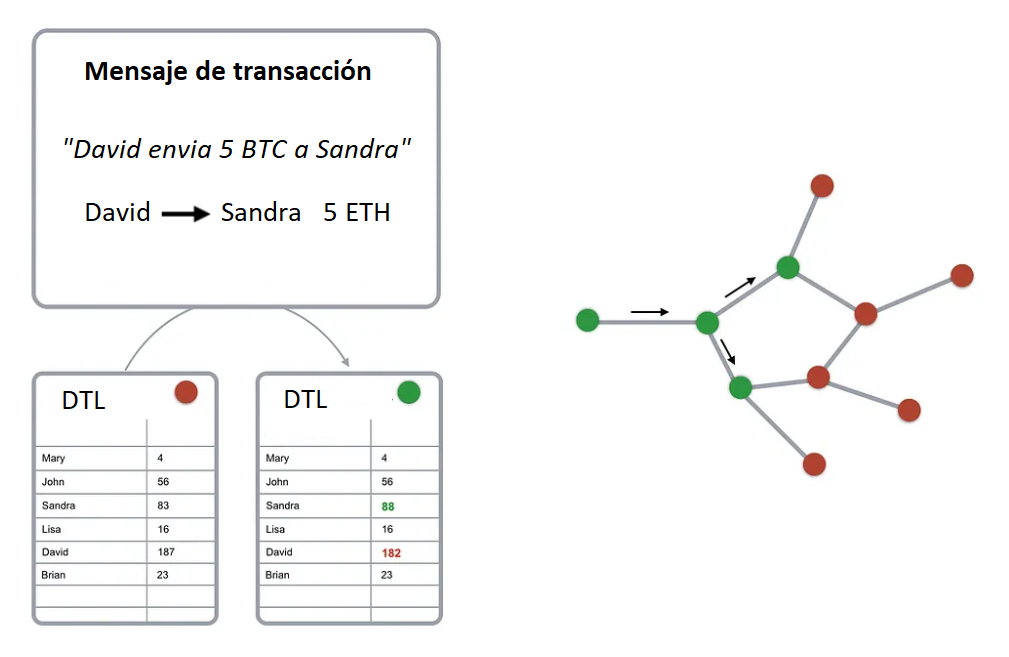
\includegraphics[width=\textwidth]{DTL}
	\caption[Libro mayor digital]{Proceso de actualización del libro mayor~\cite{BlockchainFuncionamiento}.}
	\label{fig:DTL}
\end{figure}

\subsection{Encadenamiento de bloques}

Cada bloque contiene un numero determinado de transacciones y está formado por tres elementos principales; los datos de las transacciones, el \textit{hash} del bloque anterior en la cadena  y su propio \textit{hash} único, generado a partir de la información contenida en el bloque.
Los bloques se enlazan mediante el \textit{hash} formado por los datos del bloque anterior.
El algoritmo \textit{hash} más usado en la \textit{blockchain} es SHA-256~\cite{sha256} desarrollado por la Agencia de Seguridad Nacional (NAS) en el año 1997. Es conocido por ser lento en comparación con otras funciones \textit{hash}, pero a pesar de esto destaca por su seguridad por lo que lo hace adecuado para aplicaciones financieras.
El \textit{hash} consiste en una función criptográfica que produce una salida de longitud fija a partir de una entrada de longitud variable. Cualquier cambio en el contenido de un bloque anterior requeriría recalcular todos los \textit{hashes} subsiguientes, lo cual es computacionalmente costoso y prácticamente imposible de realizar sin ser detectado.
Ver imagen \ref{fig:enlaceBloques}.

\begin{figure}[h]
	\centering
	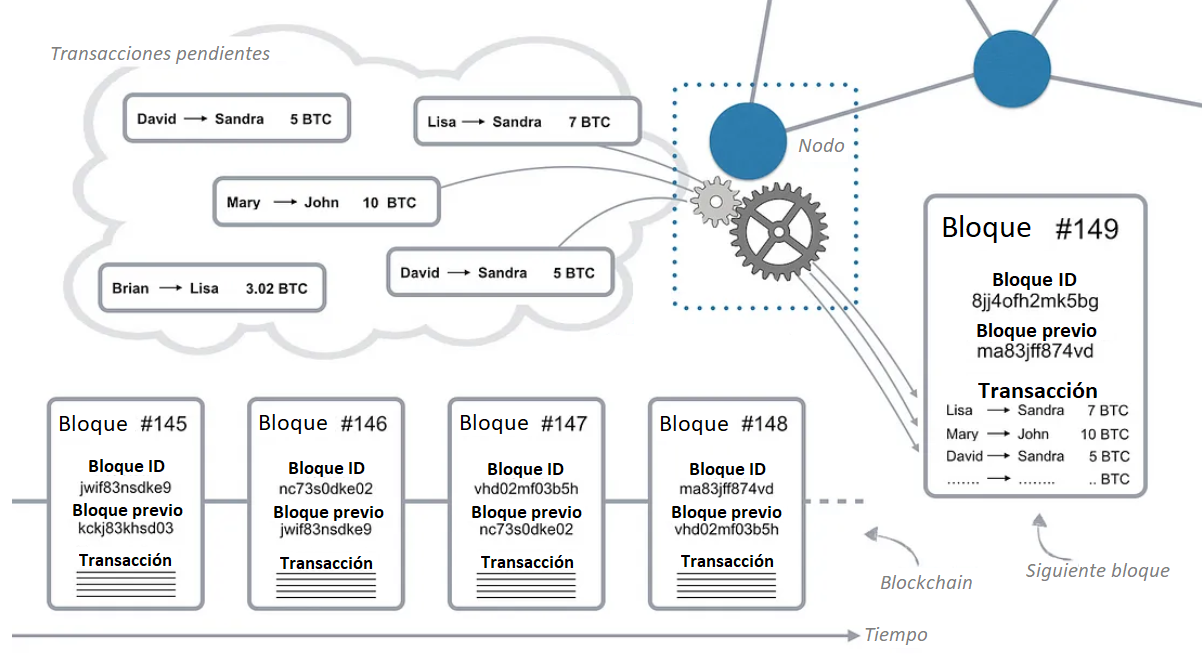
\includegraphics[width=\textwidth]{enlaceBloques}
	\caption[Encadenamiento bloques blockchain]{Encadenamiento de bloques en la \textit{blockchain}~\cite{BlockchainFuncionamiento}.}
	\label{fig:enlaceBloques}
\end{figure}

\subsection{Wallet y transacciones}

Para iniciar una transacción en la \textit{blockchain} se debe de emplear una \textit{wallet} o monedero electrónico, este es un \textit{software} que permite almacenar y intercambiar activos digitales.
Este monedero genera una y almacena un par de claves criptográficas, una clave pública que actúa como una dirección a la cual otros pueden enviar activos, y una clave privada, que se utiliza para firmar digitalmente las transacciones, asegurando que solo el propietario de la clave privada pueda autorizar la transferencia de sus activos.

Por tanto, cuando se desea realizar una transacción, el monedero electrónico firma la transacción utilizando su clave privada. Esta firma digital, generada a través de algoritmos de criptografía asimétrica como el RSA, es esencialmente un \textit{hash} criptográfico de la transacción encriptado con la clave privada del monedero.
Seguidamente, los nodos de la red al recibir la transacción, emplean la clave pública del firmante para descifrar la firma digital. Este proceso no solo autentifica que la transacción fue creada por el poseedor de la clave privada correspondiente, sino que también asegura que la transacción no haya sido modificada, ya que cualquier cambio en los datos de la transacción resultaría en una discrepancia al verificar la firma con la clave pública. Ver imagen \ref{fig:firmaDigital}.

\begin{figure}[h]
	\centering
	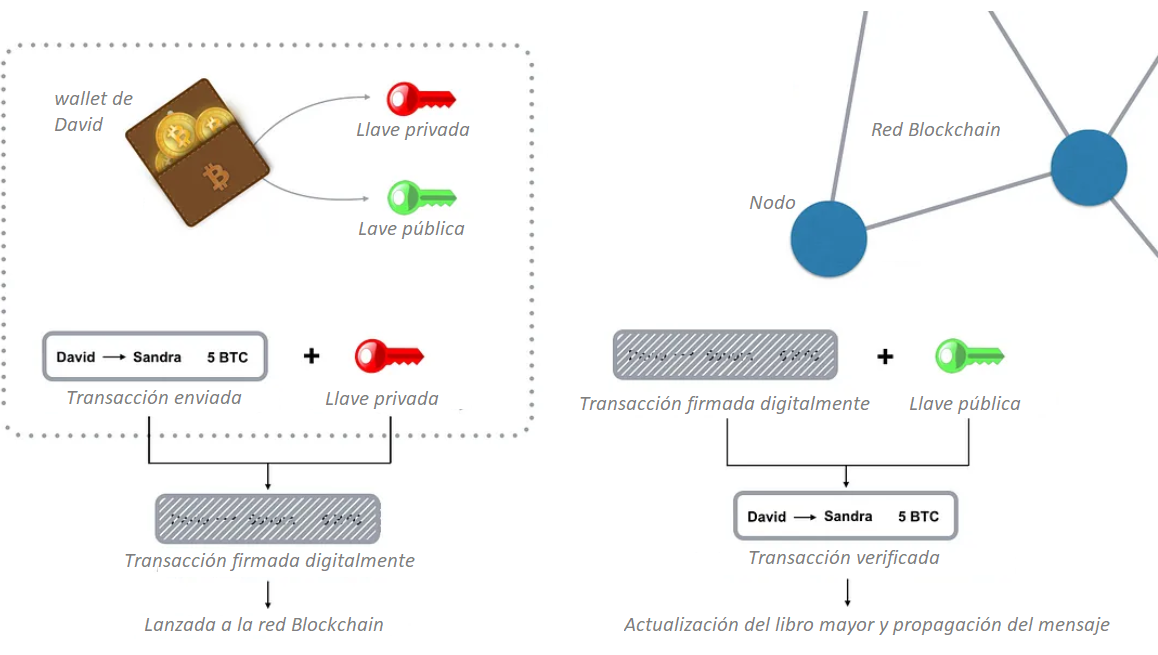
\includegraphics[width=\textwidth]{firmaDigital}
	\caption[Transacción blockchain]{Transacción encriptada con firma digital~\cite{BlockchainFuncionamiento}.}
	\label{fig:firmaDigital}
\end{figure}

A diferencia de los sistemas financieros tradicionales, la \textit{blockchain} no registra los saldos de las cuentas de manera directa. En su lugar, mantiene un registro detallado de todas las transacciones que han sido verificadas y aprobadas en la red.
Por tanto, para determinar el saldo de una \textit{wallet}, es necesario analizar y verificar todas las transacciones asociadas a ella desde la creación de la red. Este enfoque asegura que la información sea transparente y auditada constantemente por todos los nodos de la red, lo que refuerza la seguridad y la integridad del sistema.

Por tanto si un usuario quiere generar una transacción para enviar un activo, este debe generar una solicitud que incluya unas referencias llamadas \textit{inputs}, a transacciones entrantes previas que sumen la cantidad deseada. Los nodos de la red verifican estos inputs para asegurarse que no hayan sido gastados previamente.
Por ende, una vez los \textit{inputs} hayan sido referenciados, estos son invalidados para transacciones futuras, evitando el doble gasto de activos digitales.


\subsection{Consenso}

El mecanismo de consenso en una \textit{blockchain} es fundamental para mantener la integridad y la seguridad de la red. Este proceso permite que todos los nodos de la red se pongan de acuerdo sobre el estado actual del libro mayor digital, lo que significa que cualquier cambio en el \textit{blockchain} debe ser validado y aceptado por más del 50\% de los nodos de la red.

Actualmente existen dos categorías amplias de protocolos de consenso, los de finalidad probabilística, representados fundamentalmente por \textbf{Proof of work} (PoW), implica que la confirmación de una transacción se vuelve más segura a medida que se van confirmando bloques sucesivos.
Por otro lado, los protocolos con finalidad absoluta, como \textbf{Proof of Stake} (PoS) aseguran la finalización de las transacciones de manera definitiva una vez se agregan a la \textit{blockchain}.

El protocolo Proof of Work se destaca como el mecanismo de consenso más empleado en las \textit{blockchains}. En PoW, los participantes de la red, conocidos como mineros, compiten para resolver un problema criptográfico complejo, el cual requiere un considerable poder computacional. Este problema implica encontrar un valor llamado \textit{nonce}\footnote{El \textit{nonce} es un valor arbitrario que se utiliza en la minería de criptomonedas para encontrar un hash criptográfico válido bajo el protocolo Proof of Work. Es fundamental en el proceso de minería, ya que se ajusta repetidamente para generar diferentes hashes hasta que se consigue uno que cumpla con los criterios de la red.} que cuando se combina con los datos del bloque y se procesa a través de una función \textit{hash} produce un resultado que cumple con una criterio especifico, generalmente que contenga un cierto número de ceros al principio del \textit{hash}. que cuando se combina con los datos del bloque y se procesa a través de una función \textit{hash} produce un resultado que cumple con una criterio especifico, generalmente que contenga un cierto número de ceros al principio del \textit{hash}.
Este proceso, conocido como minería, garantiza que alterar un bloque ya minado sea computacionalmente inviable, proporcionando así seguridad e inmutabilidad a la cadena de bloques. A su vez, la dificultad de este problema se ajusta periódicamente para mantener un tiempo objetivo entre la creación de bloques consecutivos, asegurando la estabilidad y previsibilidad de la generación de nuevos bloques.
La labor de los mineros en la \textit{blockchain} no es altruista, este poder de cómputo es recompensado de tal manera que el primer minero en resolver el problema es recompensado con una cantidad fijada de criptomonedas~\cite{PoW}.

A pesar de su amplia adopción y probada seguridad, La minería de criptomonedas requiere de grandes granjas de minado que conllevan un elevado consumo energético teniendo un gran impacto ambiental. 
Este aspecto ha impulsado la búsqueda de alternativas más eficientes y sostenibles como el Proof of Stake (PoS) que reduce el consumo eléctrico. Este protocolo se basa en seleccionar a los validadores en proporción a la cantidad de criptomonedas que poseen y están dispuestos a bloquear como garantía.
La adopción de PoS por parte de proyectos líderes como Ethereum, con su transición a Ethereum 2.0, marca un hito importante y podría incentivar a otras criptomonedas a seguir un camino similar.

Hay que destacar que estos mecanismos de consenso únicamente son seguros en redes de una cierta magnitud ya que en contra pueden ser victimas del ataque del 51\%.
El ataque del 51\% es una vulnerabilidad en la que un único minero o grupo de mineros controla más del 50\% del poder de cómputo de la red. De tal forma que les permite influir en las confirmaciones de las transacciones, permitiendo de esta forma el fenómeno del doble gasto.
Es por esto que los mecanismos de consenso únicamente son efectivos en redes grandes, donde el tamaño de la \textit{blockchain} es equivalente a la inversión necesaria para logar un control del 51\%.




\section{Tipos de \textit{blockchain}}

Existen diferentes tipos de redes, cada una diseñada para satisfacer unas necesidades en cuanto a la privacidad, gobernanza y accesibilidad. 
Se pueden clasificar en cuatro categorías (ver tabla \ref{tab:tabla_blockchain_caracteristicas}) principales~\cite{introducciónBlockchain}:

\begin{itemize}
\item \textbf{\textit{blockchains} públicas:} Son completamente abiertas y cualquier persona puede unirse. Bitcoin y Ethereum son buenos ejemplos de \textit{blockchains} públicas, donde las transacciones y los datos son visibles para todos, manteniendo al mismo tiempo el anonimato de los usuarios. Han marcado el camino para un ecosistema de aplicaciones descentralizadas (dApps) y finanzas descentralizadas (DeFi).

\item \textbf{\textit{blockchains} semiprivadas:} Son operadas por una única entidad con la posibilidad de restringir el acceso, ofreciendo un equilibrio entre el control y la descentralización. A diferencia de las redes privadas, las semiprivadas pueden permitir la participación de partes externas bajo ciertas condiciones, manteniendo un nivel significativo de control sobre la red.
Este tipo de redes las ofrecen empresas como IBM (Hyperledger Fabric) utilizada en sectores como la salud y la financiación, permite a las organizaciones configurar redes donde los datos se comparten solo con los actores autorizados, mejorando la eficiencia y la seguridad. Ofreciendo opciones personalizables para empresas, equilibrando la privacidad con la innovación~\cite{Hyperledger}.

\item \textbf{\textit{blockchains} privadas:} Son operadas por una única organización, permiten un control total sobre quién puede participar en la red. Estas redes limitan el principio de la descentralización, pero ofrecen una solución eficaz para entornos empresariales que necesitan privacidad y eficiencia en procesos internos.
Por ejemplo, para este proyecto se ha utilizado la herramienta Ganache, la cual simula una red privada, siendo de gran utilidad en la fase de desarrollo y pruebas.

\item \textbf{Consorcio:} Representan un equilibrio entre los modelos públicos y privados, siendo operadas por un grupo de organizaciones en lugar de una única entidad. Esta posibilidad permite compartir la responsabilidad del mantenimiento de la red entre varios participantes, lo que las hace adecuadas para colaboraciones interempresariales. 
Un ejemplo real sería R3 Corda, que facilita transacciones eficientes y seguras entre instituciones financieras, reduciendo costos y tiempos de procesamiento~\cite{R3Corda}.

\end{itemize} 


\begin{table}
\small
\begin{centering}
		\begin{tabular}{@{}p{3.3cm} p{2cm} p{2.5cm} p{2.5cm} p{2.5cm}@{}}
		\toprule
		\textbf{Característica} & \textbf{Pública} & \textbf{Privada} & \textbf{Consorcio} & \textbf{Semiprivada} \\ 
		\midrule
		\textbf{Acceso} & Abierto a todos & Restringido & Restringido a organizaciones & Control selectivo \\\\
		\textbf{Descentralización} & Completa & Mínima & Parcial & Variable \\\\
		\textbf{Mecanismo de Consenso} & PoW, PoS & Permisionados & Permisionados, personalizados & Combinación \\\\
		\textbf{Transparencia} & Total & Limitada & Limitada a miembros & Configurable \\\\
		\textbf{Privacidad} & Baja & Alta & Moderada & Alta en privado \\\\
		\textbf{Velocidad y Escalabilidad} & Variable & Alta & Moderada & Configurable \\\\
		\textbf{Casos de Uso} & DApps & Registros internos & Cadena de suministro, DeFi & Compartimentos privados \\
		\bottomrule
		\end{tabular}
\end{centering}
\caption{Resumen de Tipos de \textit{blockchain} y sus Características.}
\label{tab:tabla_blockchain_caracteristicas}	
\end{table}



\section{Web3 y DApps}

Web3 emerge como una propuesta revolucionaria en la evolución de Internet, promoviendo una arquitectura descentralizada que contrasta con las fases anteriores de la web.
Desde los comienzos de Internet con Web 1.0, caracterizada por páginas estáticas y un flujo unidireccional de información, hasta la aparición de Web 2.0, que permitía a los usuarios interactuar con el contenido en línea y entre ellos. 
Sin embargo, estas etapas se han caracterizado por su centralización del poder y los datos en mano de unas pocas plataformas dominantes, lo que a menudo cuestiona preocupaciones sobre la privacidad, seguridad y monopolizción de la información~\cite{Web3}. 

En este contexto nace Web3 como una solución prometedora para abordar estas preocupaciones centrándose en descentralización. Web3 a diferencia de sus antecesoras no se limita a ser un medio para compartir y crear contenido sino que pretende redefinir las dinámicas de poder en el espacio digital mediante la implementación de tecnologías \textit{blockchain}.

La aplicación de la \textit{blockchain} más reconocida a nivel mundial ha sido \textit{Bitcoin}. Esta criptomoneda ha demostrado las capacidades de la \textit{blockchain}, permitiendo transacciones globales rápidas y seguras, caracterizadas por su alta liquidez, bajas comisiones y un nivel de anonimato que protege la privacidad del usuario~\cite{introducciónBitcoin}.

Más allá de las criptomonedas, esta tecnología se destaca por su naturaleza descentralizada, donde cada individuo en la red tiene acceso a una copia del registro completo de transacciones, lo cual garantiza una transparencia sin precedentes. Siendo así que la \textit{blockchain} cuenta con la capacidad para ofrecer la trazabilidad completa en las cadenas de suministro. Cada producto puede ser rastreado desde su origen hasta el consumidor final, asegurando la autenticidad y facilitando la detección de cualquier problema en el proceso~\cite{introducciónBlockchain}.

La seguridad es otro de los pilares fundamentales de la \textit{blockchain}, ya que la inmutabilidad del registro asegura que una vez la información ha sido añadida a la cadena, esta no podrá ser alterada, reforzando así la confianza en el sistema. 

Desde el punto de vista operativo, la \textit{blockchain} ofrece eficiencias significativas al eliminar los intermediarios, reduciendo tanto los tiempos de procesamiento como los costos asociados, a parte de minimizar las posibilidades de error.
Este aspecto es crucial en sectores como el financiero, donde los contratos inteligentes facilitan la ejecución automatizada y segura de acuerdos sin la necesidad de intermediarios, redefiniendo las prácticas comerciales y financieras en la era digital.

Dentro de este entorno de Web3, las aplicaciones descentralizadas (ver imagen \ref{fig:DAPP}) se presentan como un componente esencial, ofreciendo una alternativa a las aplicaciones centralizadas tradicionales. 
Aunque el concepto de DApp parece moderno, sus raíces se remontan más de 20 años. Las primeras aplicaciones en este ámbito fueron las aplicaciones de redes P2P, siendo algunas tan conocidas como eMule o BitTorrent, las cuales democratizaron el acceso a la información al distribuirla a través de una red de nodos (ordenadores) en lugar de centralizarla en servidores únicos~\cite{DApps}.

\begin{figure}[h]
	\centering
	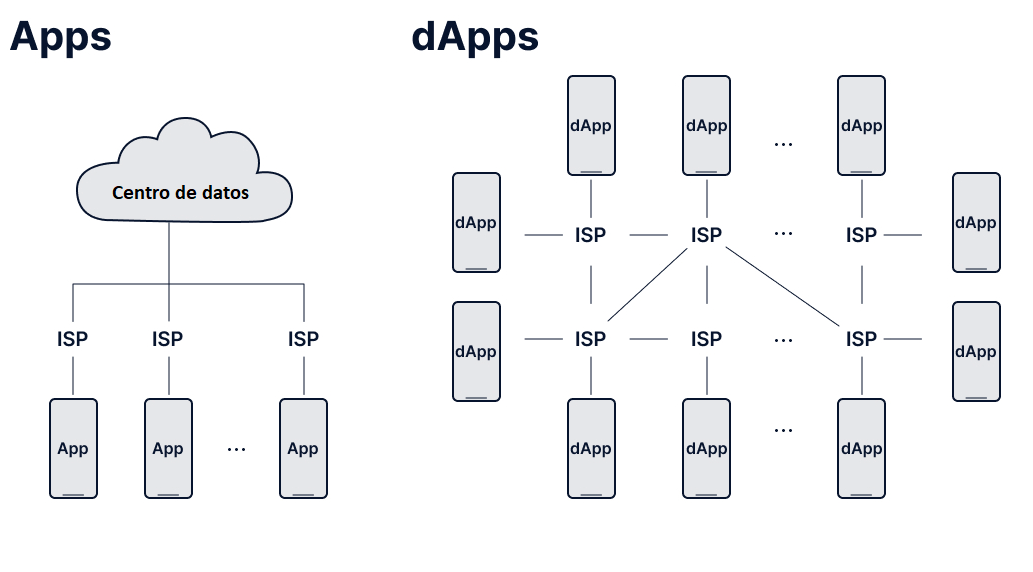
\includegraphics[width=\textwidth]{DAPP}
	\caption[Estructura de las DApps]{Estructura de las DApps~\cite{dAppDiagrama}.}
	\label{fig:DAPP}
\end{figure}

El mercado de las DApps ha experimentado un crecimiento impresionante en los últimos años, escalando de un valor de mercado de 10.5 mil millones de dolares en 2019 a más de 25 mil millones en 2022, Se espera que este mercado mantenga un crecimiento acelerado, esperándose alcanzar una capitalización de 368 mil millones en 2027. Estas cifras subrayan la creciente importancia y potencial económico de las DApps en el ecosistema digital~\cite{DAppsEconomía}.

Hoy en día las DApps adquieren una nueva dimensión, ejecutándose en redes descentralizadas y apoyándose en la tecnología de contratos inteligentes para automatizar procesos y garantizar la ejecución de acuerdos sin intermediarios.
Las Dapps destacan por su libertad y soberanía digital de los usuarios, ya que la ausencia de un punto central de control hace prácticamente imposible que se impongan restricciones arbitrarias por parte de entidades externas. A su vez, esta distribución de los datos a través de la red dificulta los ataques y manipulaciones.
Adicionalmente, el carácter de código abierto de muchas DApps fomenta la continua revisión por parte de la comunidad e incrementa la seguridad y la confianza en estas aplicaciones.

Las DApps se pueden clasificar en tres niveles distintos: 

\begin{enumerate}
\item \textbf{primer nivel}: las de primer nivel se alojan en su propia \textit{blockchain}.

\item \textbf{segundo nivel}: las de segundo nivel se alojan en \textit{blockchains} ajenas.

\item \textbf{tercer nivel}: las de tercer nivel, las cuales dependen de Dapps de segundo nivel para funcionar.
\end{enumerate}

Este proyecto se enmarca en las DApps de segundo nivel, ya que se opta por desarrollar la DApp sobre la \textit{blockchain} de Ethereum, dada su amplia aceptación y su papel predominante en el ecosistema de las aplicaciones descentralizadas.


\section{Ethereum}

Ethereum actualmente es la segunda red más grande, solo por detrás de Bitcoin y aunque normalmente se les compara, Ethereum y Bitcoin son dos proyectos totalmente distintos.
Bitcoin introdujo una forma descentralizada de dinero electrónico, permitiendo realizar transferencias en una red segura y sin intermediarios.
Ethereum por otro lado, lanzado en 2015 basándose en la base establecida por Bitcoin, expandió su funcionalidad.

La ambición de Ethereum no solo se limita a simplificar las transacciones financieras, su propósito es ampliar el alcance de las aplicaciones descentralizadas (Dapps) al proporcionar una infraestructura programable.
A diferencia de Bitcoin, no cuenta con un suministro limitado de monedas para preservar su valor, además cuenta con tiempos de minado de bloques significativamente menores, por lo que puede ofrecer una experiencia más ágil y confirmaciones de transacciones más rápidas.
Ethereum de esta manera se constituye como la columna vertebral de un Internet descentralizado(Web3)~\cite{QueEsEthereum}.

\subsection{Ether}

El Ether (ETH) es la criptomoneda que alimenta la red Ethereum, desempeña un papel fundamental tanto como activo digital como en la funcionaldiad de la red.

Similar a como ocurre con otras criptomonedas, ETH se puede enviar y recibir asegurando transacciones a cualquier parte del mundo y sin intermediarios.
A su vez, cada operación que cambie el estado de la red, supone el pago de una pequeña tarifa en ETH. Desde una simple transferencia hasta la ejecución de complejos contratos inteligentes requieren computación y almacenamiento, siendo utilizado el ETH para pagar estas denominadas "Tarifas de gas".
Finalmente como se introdujo el apartado mecanismos de consenso, Ethereum está implementando el mecanismo de consenso Proof of Stake(PoS) y el ETH constituye el activo que los participantes de la red pueden bloquear(stake) con el objetivo de dar seguridad a la red a cambio de recompensas en esta misma moneda.

Aunque ETH no tiene un suminsitro máximo fijo como Bitcoin, las políticas de emisión estan diseñadas para asegurar que el suminsitro de ETH crezca a un ritmo predecible y decreciente, lo que contribuye a la escasez y valor a largo plazo.
El valor de ETH no se basa solo en su escasez digital como en el resto de criptomonedas, también adquiere un valor adicional al permitir a los usuario pagar las tarifas de gas y más recientemente ETH se ha vuelto válido para los usuario de aplicaciones financieras descentralizadas(DEFI) al poder usarse como garantía para prestamos criptográficos o como sistema de pago~\cite{QueEsETH}.


\subsection{Ethereum Virtual Machine}

La Ethereum Virtual Machine (EVM) constituye el núcleo de la red Ethereum, proporcionando un entorno de ejecución aislado y seguro para los contratos inteligentes y las aplicaciones descentralizadas. 
La EVM es una maquina virtual turing completa, que facilita la ejecución de código en el contexto de la \textit{blockchain}.
La EVM funciona como una máquina de pila, con una profundidad de 1024 items, cada item es una palabra de 256 bits, seleccionado para su utilización con la criptografía de 256 bits.
Se ejecuta a través de códigos de operación, que realizan operaciones estándar de pila como XOR, AND, ADD, SUB, etc~\cite{QueEsEVM}.

La EVM funciona mediante la ejecución de \textit{bytecode}, un conjunto de intrucciones de bajo nivel que la máquina es capaz de interpretar y ejecutar directamente.
El bytecode se obtiene de la compilación de contratos inteligentes escritos en lenguajes de alto nivel. 
La EVM es capaz de ejecutar código en un entorno completamente aislado, por lo que los contratos pueden oprar sin comprometer la seguridad de la red. Manejando el acceso a los recursos de los computadores y limitando sus acciones en un ambiente controlado.
Esta seguridad se ve reforzada por su naturaleza descentralizada y distribuida, por lo que cualquier intento de manipulación mediante un código malicioso deberá enfrentarse al consenso de la red.
De esta forma, Ethereum funciona como un ordenador mundial descentralizado de una general en una red entre pares.

La EVM cuenta con gran flexibilidad en cuanto a su capacidad para soportar una variedad de lenguajes de programación, facilitando así la adaptabilidad del sistema Ethereum.
Además, la EVM permite que cualquier persona con acceso a Ethereum pueda desplegar sus propios contratos inteligentes, democratizando el acceso a la tecnología \textit{blockchain} y creando una gran comunidad de desarrolladores~\cite{ComoFuncionaEVM}.


\subsection{Gas}

El gas es una unidad que mide la cantidad de esfuerzo computacional requerida para ejecutar operaciones en la red Ethereum.
La tarifa de gas es la cantidad de gas usado para hacer alguna operación, multiplicado por el coste unitario del gas.
Es un mecanismo no solo de prevención contra ataques de \textit{spam}, sino tambien que facilita una economía alrededor, estableciendo un sistema de compensación para los mineros que procesan y confirman las transacciones.
El precio del gas suele expresarse en gwei, cada gwei equivale a \(0,000000001\) ETH o \(10^{-9}\) ETH.

Desde 2021 con la actualización \"London\" se introdujo el mecanismo EIP-1559, que hizo que el calculo de la tarifa de gas fuera más previsible, introduciendo los conceptos de tarifa 
base y tarifa prioritaria.

\textbf{La tarifa base} (ver tabla \ref{tab:ajuste_tarifa_base}) indica la cantidad mínima de gas a pagar para que la transacción se considere como válida para tramitar.
La tarifa base se ajusta dinámicamente bloque a bloque basándose en la ocupación del bloque anterior. El sistema, calcula cuánto gas se utilizó en total para todas las transacciones en el bloque anterior y lo compara con el tamaño de bloque previamente definido por el protocolo. Este tamaño de bloque previamente definido es una medida de cuánto gas se espera que consuman las transacciones en un bloque ideal, cada bloque en la red Ethereum tiene un tamaño esperado de 15 millones de gas.
Si el bloque anterior consumió más gas del tamaño previamente definido, la tarifa base aumentará para el siguiente bloque hasta un máximo de 12,5\%. 
El crecimiento exponencial en el costo de las transacciones cuando los bloques están constantemente sobreocupados actúa como un freno contra la congestión y alcanzando un tamaño de equilibrio de 15 millones de gas de media por bloque , ya que solo las transacciones prioritarias de aquellos que estén dispuestos a pagar más serán ejecutadas.

\begin{table}
\normalsize
\begin{centering}
	\begin{tabular}{@{}p{4em} p{5em} p{6em} p{6em}@{}}
		\toprule
		\textbf{Bloque} & \textbf{Total Gas} & \textbf{Incremento Tarifa (\%)} & \textbf{Tarifa Base (gwei)}\\ 
		\midrule
		1 & 15 M & 0\% & 100 gwei \\
		2 & 30 M & 0\% & 100 gwei\\
		3 & 30 M & 12,5\% & 112,5 gwei\\
		4 & 30 M & 12,5\% & 126,6 gwei\\
		5 & 30 M & 12,5\% & 142,4 gwei\\
		6 & 30 M & 12,5\% & 160,2 gwei\\
		7 & 30 M & 12,5\% & 180,2 gwei\\
		8 & 30 M & 12,5\% & 202,7 gwei\\
		\bottomrule
	\end{tabular}
\caption[Ajuste de la Tarifa Base Bajo Demanda]{Evolución de la Tarifa Base en Ethereum.}
\label{tab:ajuste_tarifa_base}
\end{centering}
\end{table}


Por otro lado, \textbf{la tarifa prioritaria} establece una propina que se añade a la tarifa base para que los validadores vean la transacción más atractiva para incluirla en el siguiente bloque, ya que es esta propina la que adquirirán en recompensa a su trabajo, a su vez la tarifa base es consumida y por lo tanto, eliminada.
Por lo general, la tarifa base por si sola es insuficiente para que un validador se interese por ella, por lo que la elección de una transacción por parte del validador depende de la tarifa prioritaria, la cual tiene que ajustar su precio en base al uso de la red en el momento de enviar la transacción.

Existe otro tipo de tarifa que se puede incluir de manera opcional en las transacciones, esta es la tarifa máxima, que es la que se ha usado para las transacciones dentro de este proyecto.
Este parámetro opcional recoge la cantidad máxima que el usuario está dispuesto a pagar por la validación de una transacción, por lo que dependiendo de la importancia de la transacción se puede consentir pagar más a cambio de una mayor velocidad de validación.
La tarifa total constituye la suma de la tarifa base y la tarifa prioritaria~\cite{gasEthereum}.


\subsection{Faucet}

Los \textit{faucets} representan una herramienta diseñada para facilitar a los usuarios la obtención de pequeñas fracciones de criptomonedas a cambio de realizar actividades simples, como captcha o pequeñas tareas.
El primer faucet de criptomonedas se remonta a 2010, creado por Gavin Andresen, quien entonces era el desarrollador principal de Bitcoin. Este faucet distribuyó 5 BTC a cada usuario que resolviera un \textit{captcha} simple, totalizando una entrega de 19,715 BTC~\cite{faucet}. 
Este mecanismo pretendía expandir la educación y adopción del Bitcoin entre un público más amplio.
A día de hoy los \textit{faucet} no ofrecen recompensas tan elevadas debido a la apreciación en el valor de las criptomonedas pero siguen teniendo un papel vital en la atracción y educación de nuevos usuarios mediante una vía de acceso sencilla y de bajo riesgo.

Hoy en día este enfoque se ha expandido y los \textit{faucets} se han popularizado entre las \textit{testnets}. Estos \textit{faucets} son esenciales para el desarrollo y la prueba de aplicaciones descentralizadas (dApps), facilitando un ambiente vital para la innovación y el perfeccionamiento de nuevos productos y servicios en la \textit{blockchain}.



\subsection{Contratos inteligentes}

La idea fue conceptualizada por primera vez por Nick Szabo en 1993, visionando una nueva forma de establecer acuerdos digitales. Sin embargo, la falta de una plataforma adecuada mantuvo esta idea en teoría hasta la llegada de la \textit{blockchain} con Bitcoin en 2009, y mas notablemente con Ethereum en 2014, que los contratos inteligentes se materializaron prácticamente gracias a la infraestructura que esta tecnología proporciona~\cite{smartcontractHistoria}.

Un contrato inteligente es un código que ejecuta automáticamente los términos de un acuerdo entre partes. Los códigos, almacenados en la \textit{blockchain}, son ejecutados automáticamente, cuando se cumplen unas condiciones predefinidas, haciendo cumplir un acuerdo entre dos partes no confiables sin la necesidad de un tercero de confianza.
Los contratos inteligentes utilizan la tecnología \textit{blockchain} para almacenar reglas, ejecutar automáticamente acciones cuando se cumplen esas reglas y almacenar los resultados en la \textit{blockchain}. Debido a su naturaleza inmutable y distribuida, ofrecen un nivel de seguridad y confianza superior al de los sistemas tradicionales. Así mismo, al eliminar los intermediarios, ofrecen una reducción de costos y una mayor rapidez en la ejecución de acuerdos.

Sin embargo, se enfrentan a desafíos en cuanto a cuestiones legales, la necesidad de recursos externos a la cadena de bloques, su naturaleza inmutable que dificulta la corrección de errores, problemas de escalabilidad y limitaciones del mecanismo de consenso. Las soluciones de Capa 2, como la Lightning Network y Ethereum Plasma, se diseñaron para abordar los desafíos de escalabilidad y eficiencia de las \textit{blockchain} de Capa 1. Operan sobre la cadena principal para permitir transacciones más rápidas y con menores costos, manteniendo la seguridad y descentralización~\cite{AplicacionesDesafiosSmartcontract}.



\section{\textit{Tokenización}}

La \textit{tokenización}~\cite{tokenización} es el proceso de convertir la información delicada o activos del mundo real en representaciones digitales denominadas \textit{tokens}, dentro del ecosistema \textit{blockchain}.
Este procedimiento juega un papel crucial en la protección de datos confidenciales al reemplazar la información original con un \textit{token} único, el cual no tiene valor fuera de su contexto específico de uso.

La información sensible se almacena en la `bóveda de \textit{tokenización}'~\cite{bóvedaTokenización} una infraestructura de almacenamiento segura donde los datos originales se cifran y aíslan. El acceso a la bóveda es solo posible a través de rigurosos controles de seguridad y claves de descifrado específicas.
A diferencia de los métodos de cifrado que utilizan un algoritmo matemático para transformar datos en un formato ilegible que puede ser revertido usando un clave concreta, la \textit{tokenización} no mantiene una relación algorítmica con los datos originales. En consecuencia, los \textit{tokens} generados no pueden ser revertidos sin un acceso autorizado a la bóveda de \textit{tokenización}, lo que proporciona una capa adicional de seguridad.
Por lo tanto, mientras los datos originales se almacenan en una bóveda de \textit{tokens} segura, los \textit{tokens} se distribuyen en sistemas internos para su utilización diaria.

Un elemento importante de los \textit{tokens} es que, fuera de la relación financiera específica para la que fueron creados, carecen totalmente de valor. Ya que una función de los mismos es representar un valor específico en una relación determinada. Esta característica los distingue de las criptomonedas y otros activos digitales que pueden tener un valor en el mercado abierto.
En el ámbito de los pagos y transacciones, los \textit{tokens} permiten a las organizaciones procesar transacciones y almacenar información de clientes sin exponer los datos críticos a riesgos de seguridad.
La generación de un \textit{token} se realiza mediante contratos inteligentes en la \textit{blockchain}, que definen las reglas y la lógica para su emisión, transferencia y anulación. Los contratos inteligentes aseguran que el token sea único y esté vinculado de manera inmutable a los datos o activos correspondientes en la bóveda.

En el ecosistema \textit{blockchain} existen diversos tipos de tokens diseñados para propósitos específicos~\cite{tiposToken}:

\begin{itemize}
\item \textbf{Tokens de Seguridad:} Representa inversiones digitales en activos reales como acciones o bonos, respaldado por activos tangibles y regulado por entidades gubernamentales.
\item \textbf{Tokens de Gobernanza:} Permiten a los poseedores participar en la toma de decisiones dentro de una plataforma o protocolo, votando en cambios o propuestas.
\item \textbf{Tokens de Utilidad:} Proporciona acceso a productos o servicios dentro de una plataforma \textit{blockchain}, sin ser considerado un valor financiero.
\item \textbf{Tokens Comunitarios:} Recompensan la participación en una comunidad, ofreciendo beneficios como acceso exclusivo o descuentos a los miembros activos.
\item \textbf{Tokens Vinculados a valores:} Son digitales pero están respaldados por activos físicos como metales preciosos, permitiendo a los inversores negociar activos reales de manera digital.

\end{itemize}

Todos los tipos de tokens existentes se pueden clasificar en dos grandes grupos, los tokens fungibles y los tokens no fungibles.


\subsection{Tokens fungibles}

La definición de fungibilidad es esencial para entender los aspectos fundamentales de un token fungible. Tomando como referencia una definición ofrecida por el Tesoro Público del Gobierno de España, la fungibilidad se describe como la `Propiedad de un conjunto de valores que los hace plenamente equivalentes entre sí a efectos legales'~\cite{fungibilidadGob}.
La fungibilidad es un concepto que nos rodea en la vida cotidiana, siendo el dinero uno de los mejores ejemplos. Cuando se intercambia un billete de cinco euros por otro billete de cinco euros, se entiende que ambos tienen el mismo valor y son aceptados de la misma manera.

Este principio se puede extrapolar al mundo digital y a la \textit{blockchain}. Los token fungibles actúan de forma similar al dinero físico, siendo indistinguibles y equivalentes entre unidades del mismo tipo.
El ejemplo más conocido es Bitcoin, convirtiéndolo en una herramienta poderosa para las transacciones digitales.


\subsection{Tokens no fungibles (NFT)}

Los NFT han emergido como una innovación disruptiva en el ámbito del comercio electrónico, especialmente en el mundo del arte digital.
A diferencia de los tokens fungibles, cada NFT es una certificación criptográfica que contiene información y códigos de identificación únicos que los hacen irremplazables e intercambiables.
Esta característica los hace particularmente adecuados para representar activos digitales únicos y derechos de propiedad en el mundo digital.
En el contexto de los contratos laborales, los NFT pueden ser utilizados para \textit{tokenizar} y asegurar la autenticidad de contratos individuales, garantizando que los términos acordados sean únicos y vinculados inequívocamente a las partes involucradas~\cite{NFTintroducción}.


\subsubsection{ERC-721}

ERC-721 es un estándar propuesto por el desarrollador Dieter Shirley a finales de 2017 que introdujo el concepto de tokens no fungibles en la red Ethereum~\cite{ERC721Introducción}.
Abriendo las puertas a una nueva dimensión de activos digitales únicos, a diferencia de los tokens fungibles basados en el estándar ERC-20.

La creación del estándar ERC-721 fue motivada por la creciente demanda de tokens digitales que pudieran representar de manera única activos individuales.
La singularidad de los tokens ERC-721 les dota de gran utilidad en aplicaciones donde el ámbito de autenticidad y la propiedad exclusiva son cruciales.
Su uso mas popular se enfoca en el mundo del arte, asegurando la autenticidad y unicidad de diferentes obras, aunque también ha tomado gran relevancia en el ámbito legal. 
Poniendo de ejemplo este proyecto, con el uso del estándar ERC-721 se puede \textit{tokenizar} y autenticar contratos laborales, asegurando la transparencia y la inmutabilidad de los términos acordados, verificando el cumplimiento de los acuerdos.

Este estándar cuenta con una serie de propiedades técnicas que lo hacen versátil. Algunas de estas propiedades son la asignación de un nombre, la definición de un balance de tokens dentro de una dirección y la implementación de funciones que permiten la transferencia segura de la propiedad.


\capitulo{4}{Técnicas y herramientas}


\section{Herramientas}

Se muestra a continuación las herramientas usadas a lo largo del desarrollo del proyecto.

\subsection{React Native}

La elección del framework adecuado juega un papel crucial en el éxito de un proyecto. Dicha elección se complica aún más cuando se carece de experiencia previa en el desarrollo de aplicaciones móviles. Dentro del gran abanico de posibilidades React Native y Flutter emergen como grandes líderes en el sector gracias a sus grandes comunidades y la abundancia de recursos en línea. Por otro lado se pueden descartar directamente frameworks como Swift debido a su exclusividad para aplicaciones para iOS debido a que el objetivo de este proyecto es desarrollar una aplicación para Android.

React Native se presenta como mi elección favorita, este es un framework de código abierto creado por Facebook orientado a la creación de aplicaciones nativas tanto en iOS como en Android. React Native esta basado en JavaScript y React, una biblioteca de JavaScript destinada a la creación de interfaces de usuario. Fue lanzado en 2015 con el propósito de superar las limitaciones del desarrollo de aplicaciones móviles basado solo en HTML5, en las que simplemente se adapta aplicaciones web a un entorno móvil. React Native utiliza componentes nativos en lugar de WebViews para la interfaz de usuario, esto conlleva a que las aplicaciones se sientan y actúen como en una aplicación nativa. Uno de los elementos mas importantes de este framework es el "React Native Bridge", el cual facilita la comunicación entre el código JavaScript y los elementos nativos del dispositivos. El puente maneja de forma paralela dos flujos de trabajo, uno ejecuta la lógica de la aplicación en JavaScript y otro gestiona las operaciones de la interfaz de usuario nativa. Esto permite que las aplicaciones en React Native accedan a las características del dispositivo como la cámara o la ubicación manteniendo una experiencia fluida para el usuario. 

Mi preferencia de este framework sobre el resto radica en mi familiaridad previa con la programación web y JavaScript, lo cual reducirá la curva de aprendizaje en la transición hacia React Native en contraste con otros frameworks que podrían requerir el aprendizaje de nuevos lenguajes de programación o paradigmas de programación. Por otro lado, uno de los grandes motivos de este framework es su gran popularidad, el cual se traduce en un gran riqueza de recursos disponibles, como bibliotecas, videotutoriales o foros, crucial a la hora de enfrentar los desafíos que puedan surgir. Finalmente aunque para este proyecto no sea un requerimiento hay que tener en cuenta la gran versatilidad de React Native, el cual permite la creación de aplicaciones nativas tanto en Android como en iOS a partir de un único código base. Optimizando así el proceso de desarrollo permitiendo en un futuro poder dar cobertura a un mercado más amplio sin esfuerzos duplicados.

Como había nombrado anteriormente Flutter es otro framework que destaca sobre el resto y ofrece ciertas ventajas notables sobre Reac Native, como un rendimiento superior gracias al uso de su motor de renderizado propio y la gran capacidad de personalización de la interfaz de usuario. Aunque Flutter pudiera ser superior en algunos aspectos técnicos sigo decantándome por React Native debido a su gran comunidad y la familiaridad que tengo con las tecnologías web, priorizando así un aprendizaje más sencillo frente a posibles mejoras en el rendimiento. Por otro lado existen frameworks Ionic y Xamarin que los he descartado debido a sus limitaciones en términos de acceso a funciones nativas o una comunidad bastante inferior comparado con React Native o Flutter. Kotlin era un opción con gran potencial para el desarrollo nativo de aplicaciones Android pero la descarte rápidamente debido a que disponía de una curva de aprendizaje más pronunciada que su competencia y iba a representar un obstáculo significativo en cuanto al tiempo de desarrollo sin garantizar beneficios proporcionales a dicho esfuerzo.

Respecto a Angular, si bien este framework ofrece un ecosistema robusto para el desarrollo de aplicaciones web dinámicas y complejas utilizando TypeScript, es importante mencionar que también es posible desarrollar aplicaciones móviles con Angular, ofreciendo una experiencia cercana a la nativa, aunque a través de un enfoque diferente al de las aplicaciones nativas desarrolladas con React Native. Sin embargo, para el desarrollo específico de aplicaciones móviles nativas, React Native encaja mejor con los objetivos del proyecto.
Angular no deja de ser una elección excelente, pero debido a la preferencia del proyecto de enfocarse en una aplicación móvil sin la necesidad de dar soporte de navegador, Angular puede no ser la opción más adecuada para el proyecto.
Por lo tanto he descartado Angular buscando una solución más enfocada y optimizada para el desarrollo móvil, aprovechando las capacidades nativas de los dispositivos móviles.


\subsection{Expo}

Expo es un conjunto de herramientas, librerías y servicios para desarrollar aplicaciones nativas utilizando en Javascript y React Native. Proporciona un entorno de trabajo rico en funcionalidades que evita las complicaciones asociadas con la configuración nativa.
Expo ha sido fundamental en el proyecto para desarrollar la interfaz de usuario permitiendo probar y visualizar cambios en tiempo real en diferentes plataformas.
Una de las funcionalidades significativas de Expo ha sido su capacidad para facilitar la ejecución y testeo de la aplicación directamente en dispositivos móviles personales sin necesidad de emuladores. Esto se logra únicamente descargando la aplicación ExpoGo en el teléfono móvil y escaneando un código QR generado por el entorno de desarrollo Expo.
Expo tiene un papel fundamental en las fases de prueba y depuración, permitiendo probar la aplicación en un entorno real y ajustar la interfaz la interfaz de usuario con un ciclo de retroalimentación casi instantáneo.


\subsection{Solidity}

Solidity es un lenguaje de programación orientado a objetos de alto nivel diseñado para escribir Smart Contracts que se ejecutan en la Ethereum Virtual Machine (EVM). Solidity consta de una sintaxis similar a lenguajes como JavaScript, C++ y Python, lo que facilita su aprendizaje. Es un lenguaje de tipado estático, lo que significa que el tipo de cada variable se define y no cambia durante al ejecución del contrato.
Una de las potencialidades más destacadas de Solidity es su soporte para la herencia, una característica común en la programación orientada a objetos. Esto permite que los Smart Contracts hereden propiedades y comportamientos de otros contratos, beneficiándose de la reutilización de código y la organización de la lógica del mismo. En mi caso de gran utilidad para utilizar las funcionalidades del estándar ERC721 proporcionado por OpenZeppelin, que ofrece un conjunto de contratos inteligentes auditados y aprobados por su comunidad.


\subsection{Remix}

Remix es un entorno de desarrollo integrado (IDE) diseñado para el desarrollo de Smart Contracts escritos en Solidity. Proporciona una interfaz accesible y fácil de usar para escribir, compilar, probar y desplegar Smart Contracts directamente desde el navegador, sin la necesidad de instalar software adicional.
Remix también ofrece funcionalidades avanzadas como la compilación en tiempo real, el despliegue de contratos en diversas redes de prueba (testnets) y la interacción con SmartContracts ya desplegados.
Una de las características más útiles de este IDE es su análisis estático del código, pudiendo así identificar posibles errores de programación o vulnerabilidades de seguridad. Crucial para el desarrollo de Smart Contracts donde los errores pueden suponer consecuencias financieras significativas.
Además, Remix se integra con herramientas y plugins adicionales, ofreciendo un entorna mas rico y extenso permitiendo conectarse con herramientas y servicios como MetaMask, Truffle y Ganache ampliamente utilizados en mi proyecto.
Remix ha tenido una gran protagonismo en el desarrollo de mi proyecto permitiéndome iterar rápidamente a través de diferentes versiones de contratos inteligentes. Pudiendo ejecutar pruebas unitarias con diversas redes Ethereum como Rinkeby y Goerli, indispensable para validar la lógica del Smart Contract antes de su despliegue final. Dándome una gran capacidad de testeo en un entorno controlado pero realista el cual ha sido crucial para la corrección de errores y la optimización del uso de gas, asegurando así la eficiencia y seguridad de los contratos inteligentes desarrollados.


\subsection{Truffle}

Tras una fase inicial de desarrollo de los Smart Contracts usando Remix, la transición al uso de Truffle ha marcado un punto de inflexión en la complejidad de mi proyecto.
Truffle consiste en una suite de desarrollo avanzada para Ethereum, ofreciendo un conjunto de herramientas diseñadas para facilitar el desarrollo, gestión y despliegue de Smart Contracts.
Truffle proporciona un entorno de desarrollo estructurado generando una jerarquía de carpetas para favorecer la implementación de proyectos blockchain complejos.
Ahorra mucho tiempo con su sistema de migraciones y scripts de despliegue el cual automatiza y simplifica el proceso de lanzamiento de contratos.
Aunque Remix es una excelente herramienta, Truffle eleva la posibilidad de hacer pruebas unitarias a otro nivel con un marco de prueba mucho mas sofisticado, permitiendo ejecutar test en Solidity o JavaScript.
Finalmente, uno de las mayores ventajas de usar Truffle en el desarrollo de aplicaciones descentralizadas es en cómo simplifica el proceso de unir el trabajo que se realiza en el backend con el frontend. Cuenta con herramientas que ayudan a conectar Smart Contracts con aplicaciones móviles haciendo que la conexión sea mas directa y menos propensa a errores.


\subsection{OpenZeppelin}

OpenZeppelin es una biblioteca para el desarrollo seguro de Smart Contracts en Ethereum. Ofrece implementaciones auditadas y probadas para minimizar riesgos de seguridad.
Su uso ha sido crucial para el desarrollo de mi proyecto, usando el estándar ERC721 para la representación de los contratos como tokens no fungibles (NFTs) asegurando que la aplicación cumpla con los estándares de seguridad.


\subsection{Ganache}

Ganache funciona como un nodo de Ethereum personal, permitiendo a los desarrolladores simular un entorno de blockchain que opera localmente ofreciendo un espacio seguro y controlado para experimentar sin ningún costo real ni tiempos de espera con las redes públicas de Ethereum.
Proporciona diez cuentas cargadas con 1000 ETH cada una y con su clave pública y privada correspondiente.
Ganache se puede usar tanto en la línea de comandos como en en la aplicación de escritorio y proporciona  una vista de las transacciones, bloques y estado de la red, mostrando el feedback en tiempo real, vital para realizar una iteración rápida.
Ganache se integra perfectamente con Truffle, siendo Ganache el entorno de desarrollo local predeterminado de Truffle.


\subsection{MetaMask}

MetaMask es una extensión de navegador y una aplicación móvil que permite a los usuarios interactuar con la blockchain de manera segura y sencilla. Actúa como puente entre los navegadores web y la blockchain.
Su funcionamiento es análogo a una cartera digital, permitiendo a los usuarios almacenar sus cuentas de Ethereum.
Al conectarse a dApps, los usuarios pueden usar sus cuentas de MetaMask para autenticarse eliminando la necesidad de copiar claves privadas manualmente. Por otro lado, aplica una capa adicional de seguridad ya que esta herramienta encripta la información del usuario y almacena las claves privadas directamente en el dispositivo del usuario. Esto asegura que solo el usuario tenga acceso a sus fondos y datos.
La integración de MetaMask en mi proyecto no solo mejora la experiencia del usuario final, sino que también agiliza el desarrollo de mi proyecto al proporcionar una manera fácil y segura de acceder a los activos de los usuarios.


\subsection{Node.js}

Node.js es un entorno de ejecución en JavaScript, tradicionalmente un lenguaje de programación del lado del cliente, para desarrollar aplicaciones del lado del servidor. Es conocido por su capacidad para manejar operaciones asíncronas y por su escalabilidad siendo de gran popularidad en el desarrollo de aplicaciones web modernas. Una de las ventajas de de Node.js es su ecosistema de paquetes gestionados por npm (Node Package Manager), que proporciona acceso a miles de librerías.
En el proyecto se ha usado de manera frecuente, más allá de ser un requisito para utilizar Truffle, a través del uso de npm install se ha usado "npm install" para descargar librerías y paquetes necesarios para el desarrollo del frontend y backend.
Bien es así, que aunque React Native sea el framework principal del desarrollo del frontend, la gestión de sus dependencias, librerías adicionales se realiza mediante npm, el cual opera sobre Node.js.
A su vez, por ejemplo el uso de la biblioteca Web3.js, una de las mas importantes del proyecto ya que es fundamental para interactuar con la blockchain, se ha instalado y gestionado usando npm.
Por tanto, Node.js ha sido una pieza crucial en el desarrollo del proyecto, simplificando la configuración del proyecto.


\subsection{Mendeley}
\capitulo{5}{Aspectos relevantes del desarrollo del proyecto}

Este apartado pretende recoger los aspectos más interesantes del desarrollo del proyecto, comentados por los autores del mismo.
Debe incluir desde la exposición del ciclo de vida utilizado, hasta los detalles de mayor relevancia de las fases de análisis, diseño e implementación.
Se busca que no sea una mera operación de copiar y pegar diagramas y extractos del código fuente, sino que realmente se justifiquen los caminos de solución que se han tomado, especialmente aquellos que no sean triviales.
Puede ser el lugar más adecuado para documentar los aspectos más interesantes del diseño y de la implementación, con un mayor hincapié en aspectos tales como el tipo de arquitectura elegido, los índices de las tablas de la base de datos, normalización y desnormalización, distribución en ficheros3, reglas de negocio dentro de las bases de datos (EDVHV GH GDWRV DFWLYDV), aspectos de desarrollo relacionados con el WWW...
Este apartado, debe convertirse en el resumen de la experiencia práctica del proyecto, y por sí mismo justifica que la memoria se convierta en un documento útil, fuente de referencia para los autores, los tutores y futuros alumnos.

\capitulo{6}{Trabajos relacionados}

\section{OpenLaw}

\href{https://www.openlaw.io/}{OpenLaw} es una plataforma que combina contratos inteligentes con protocolos legales convencionales.
Desarrollada para mejorar la eficiencia, seguridad y transparencia en la gestión de acuerdos legales, OpenLaw se posiciona en la vanguardia de la intersección entre la ley y la tecnología blockchain.

La plataforma usa la red Ethereum para registrar cada contrato  en la \textit{blockchain} garantizando que una vez el contrato es firmado, este permanezca inalterable minimizando las posibles disputas sobre el y permitiendo una ejecución automática de los términos acordados.

OpenLaw integra tecnologías de firma digital, facilitando la ratificación de acuerdos sin necesidad de encuentros físicos.
En regiones donde los contratos inteligentes y las firmas digitales están legalmente reconocidos, OpenLaw ofrece una herramienta poderosa y conforme a la ley. Sin embargo, en jurisdicciones sin una regulación clara sobre el uso de la tecnología \textit{blockchain} en el ámbito legal, puede existir incertidumbre sobre la validez y ejecución de estos acuerdos.

En la imagen \ref{fig:openLawExample} se puede observar como se ratificaría un contrato usando OpenLaw.

\begin{figure}[h]
	\centering
	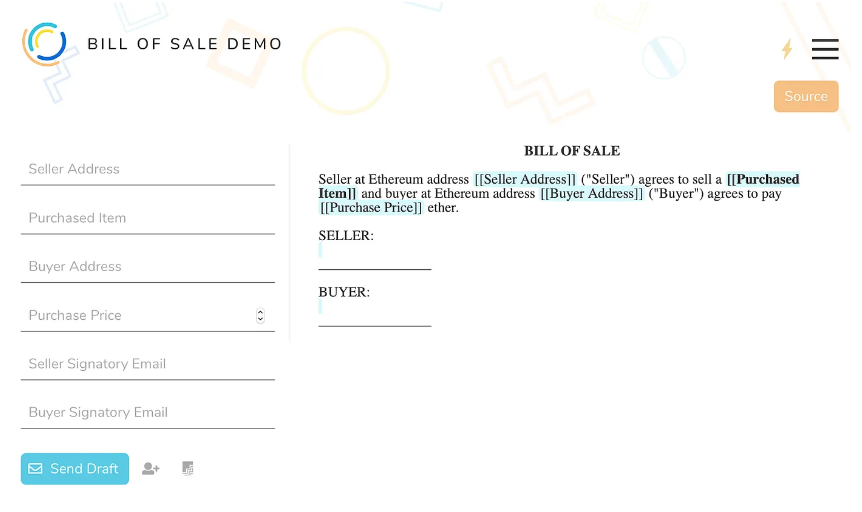
\includegraphics[width=\textwidth]{openLawExample}
	\caption[Ejemplo OpenLaw]{Ejemplo de contrato vinculante usando OpenLaw.}
	\label{fig:openLawExample}
\end{figure}

\section{Proyectos}

\subsection{TFG - Aplicación web para operar con contratos digitales a través
de blockchain}

El trabajo de Francisco Javier Gozalo Cervera~\cite{tfgSmartContacts} se enfoca en desarrollar una aplicación web destinada a la gestión y operación de contratos digitales utilizando tecnología blockchain.

Su proyecto aborda una necesidad similar al presente trabajo, pero difiere significativamente en su enfoque y ejecución. Gozalo Cervera ha desarrollado una aplicación diseñada específicamente para navegadores web, donde los contratos son creados inicialmente en formato PDF y luego son almacenados en la blockchain para asegurar su integridad y seguridad.

Esta plataforma proporciona una interfaz accesible que permite a los usuarios gestionar sus contratos de manera eficiente y segura, utilizando estándares robustos de tecnología blockchain para garantizar la confiabilidad de los documentos digitales.
\capitulo{7}{Conclusiones y Líneas de trabajo futuras}

Todo proyecto debe incluir las conclusiones que se derivan de su desarrollo. Éstas pueden ser de diferente índole, dependiendo de la tipología del proyecto, pero normalmente van a estar presentes un conjunto de conclusiones relacionadas con los resultados del proyecto y un conjunto de conclusiones técnicas. 
Además, resulta muy útil realizar un informe crítico indicando cómo se puede mejorar el proyecto, o cómo se puede continuar trabajando en la línea del proyecto realizado. 


\section{Conclusiones}

Tras la realización del proyecto, se logró desarrollar una aplicación móvil que implementa una solución basada en \textit{blockchain} y contratos inteligentes que aborda eficientemente los problemas de la economía sumergida.
Este proyecto ha sido una experiencia enriquecedora, permitiéndome familiarizarme con diversas tecnologías y herramientas que no había utilizado previamente.
Durante el desarrollo aprendí a programar Solidity y React Native y a usar Expo para el desarrollo de aplicaciones móviles. Además profundicé en el uso y funcionamiento con la \textit{blockchain} y mi familiaricé con herramientas como Firebase.

A lo largo del proyecto, me he encontrado diversas dificultades, muchas de las cuales se vieron acentuadas debido a mi falta de experiencia con algunas de las tecnologías. El uso de la \textit{blockchain} real presentó varios desafíos técnicos, especialmente en la integración con la aplicación Android. La conexión y uso de MetaMask que es relativamente sencillo en aplicaciones web, resultaron ser bastante más difícil en el entorno móvil.

A pesar de los desafíos y contratiempos, estoy satisfecho con el resultado final del proyecto. La experiencia fue extremadamente valiosa y me permitió aprender sobre múltiples tecnologías que tienen aplicaciones prácticas significativas.

\section{Lineas de trabajo futura}

El proyecto todavía tiene mucho potencial para crecer aún más, por lo que existen diversas mejoras que se podrían incorporar en futuros desarrollos. No cabe duda de que la principal línea futura de trabajo, contando con un pequeño presupuesto, debe ser desplegar el contrato en una red \textit{blockchain} real.
Implementar el contrato en una red real permitirá que la aplicación funcione en un entorno de producción, asegurando la conectividad entre la aplicación móvil y la \textit{blockchain}.
Del mismo modo, otro objetivo es lanzar la aplicación al mercado global, publicando la aplicación en tiendas de aplicaciones como Google Play, proporcionando mayor seguridad y confianza a los usuarios.

Aprovechando las funcionalidades que soportan los dispositivos móviles, sería interesante incorporar nuevas características como filtros de búsqueda avanzados y servicios de geolocalización.
Los filtros de búsqueda permitirían al usuario buscar contratos según diferentes criterios como ubicación, duración y salario, haciendo la búsqueda de contratos más eficiente.
Por otro lado, la implementación de geolocalización podría registrar automáticamente las horas de trabajo del empleado, asegurando el cumplimiento del contrato y facilitando la precisión en el pago del salario. Además, la geolocalización mejoraría la seguridad y transparencia del contrato, proporcionando un registro claro y verificable de las horas trabajadas.




\bibliographystyle{plain}
\bibliography{bibliografia}

\end{document}
